\documentclass[prc,amsmath,twocolumn,superscriptaddress]{revtex4}
%\bibliographystyle{prsty}
\usepackage{gensymb}
\usepackage{graphicx,color}
\usepackage{amssymb}
\usepackage{enumerate}
\usepackage{verbatim}
\usepackage{natbib}


\begin{document}
  \newcommand {\nc} {\newcommand}
  \nc {\Sec} [1] {Sec.~\ref{#1}}
  \nc {\IR} [1] {\textcolor{red}{#1}} 

\title{Gauss elimination}


\author{Alaina~Ross}

\date{\today}

%%%%%%%%%%%%%%%%%%%%%%%%%%%%%%%%%%%%%%%%%%%%%%%%%%%%%%%%%%%%%%%%%%%%%%%%%%%%%%%%%%%%%%%%%%%%%%%%%%%%%%%%%%%%%%%%%%%%%%%%%%%%%%%%%%%

\begin{abstract}
 %\noindent {\bf Background:} Systems of equations are often solved via matrix equations and Gauss elimination. If the necessary matrices are large enough then the calculation is performed computationally. \\
 %{\bf Purpose:} The goal of this work is to parallelize a Gauss elimination code to determine the performance limits and test different parallel implementations. \\
 %{\bf Method:} We use both OpenMP and MPI parallelism separately and inspect their time to solution for varying matrix sizes and number of threads/processes. \\
 %{\bf Results:} We find the OpenMP implementation to be both simpler and better performing, while the MPI implementation has too much communication overhead for much performance increase. \\
 %{\bf Conclusions:} Our results demonstrate the importance of choosing the right form of parallelism for the given algorithm, in this case shared memory parallelism is the right choice.
\end{abstract}


\maketitle

%%%%%%%%%%%%%%%%%%%%%%%%%%%%%%%%%%%%%%%%%%%%%%%%%%%%%%%%%%%%%%%%%%%%%%%%%%%%%%%%%%%%%%%%%%%%%%%%%
\section{introduction}
\label{intro}
Often in science problems can be written as a linear second order differential equation such as:
\begin{equation}
\frac{d^2y}{dx^2}+k^2(x)y=f(x).
\end{equation}
One specific example of this is the Poisson equation in electromagnetism, which is used to find the electrostatic potential, $\Phi$, from a spherically symmetric charge distribution, $\rho (r)$ as:
\begin{equation}
\nabla^2\Phi=\frac{1}{r^2}\frac{d}{dr}\left(r^2\frac{d\Phi}{dr}\right)=-4\pi \rho(r)
\end{equation}
using the substitution $\Phi=\phi/r$ and simplifying gives:
\begin{equation}
-\frac{d^2\phi}{dr^2}=4\pi r \rho(r).
\end{equation}

In general terms, the equation we aim to solve is $-u''(x)=f(x)$. Since this is a second order differential equation, it requires two boundary conditions. Here we use Dirchilet conditions, namely $u(0)=u(1)=0$. \\

Turning these continuous functions in discrete ones we can approximate the second derivative as:
\begin{equation}
-\frac{u_{i+1}+u_{i-1}-2u_i}{h^2}=f_i \quad i=1,2...n
\label{deriv}
\end{equation}
where $h$ is the step size defined as $h=1/(n+1)$ and n is the number of grid points. This set of equations then can be rearranged as a matrix equation $\hat{A}\vec{u}=\vec{b}$ where:
\begin{equation}
\hat{A}=\begin{bmatrix} a_{1,1} & a_{1,2} &a_{1,n} \\ a_{2,1}  & a_{2,2} &a_{2,n} \\ a_{n,1}  & a_{n,2}  &a_{n,n} \end{bmatrix}
\quad \vec{u}=\begin{bmatrix} u_1  \\ u_2\\ u_n \end{bmatrix} 
\quad \vec{b}=\begin{bmatrix} h^2f_1  \\ h^2f_2\\ h^2f_n \end{bmatrix}
\end{equation}

To solve this matrix equation the first goal is to get the matrix in row echelon form (shown below), where the only nonzero elements form the upper right triangle of the matrix. This step is called forward elimination and is done analytically via elementary row operations i.e. addition, interchanging rows, and multiplication by a constant.

\begin{equation}
\begin{bmatrix} a_{1,1} & a_{1,2} &a_{1,n} \\ 0  & \tilde{a}_{2,2} &\tilde{a}_{2,n} \\ 0  & 0  &\tilde{a}_{n,n} \end{bmatrix}
\begin{bmatrix} u_1  \\ u_2\\ u_n \end{bmatrix}=\begin{bmatrix} \tilde{b}_1  \\ \tilde{b}_2\\ \tilde{b}_n \end{bmatrix}
\label{reduced}
\end{equation}

Algorithmically, this can be calculated two ways: the simpler way which only uses addition and multiplication by a constant but will fail if $a_{i,i}$ = 0, or the more sophisticated way where rows are interchanged to ensure a solution even when $a_{i,i}$ = 0~\cite{book}. In this work we will use the former method and simply ensure that for all matrices $a_{i,i}$ $\neq$ 0. \\

In this work we implement gauss elimination for a general matrix as well as for a tridiagonal matrix and study the performance characteristics and numerical accuracy of each for matrix sizes of $n=10,100,1000$. In addition, we compare the performance of our solutions to that of a more sophisticated algorithm known as LU decomposition in order to determine the most efficient algorithm for the problem at hand. In Section~\ref{methods}, the implementation of the various algorithms are described. In Section~\ref{results} the performance and accuracy of the code are analyzed. Finally, in Section~\ref{conc} we give a summary and our conclusions.

\section{methods}
\label{methods}
To begin the Gauss elimination we implement the arrays using the matrix and vector classes in the armadillo library [cite]. We then start with the first row and column of the matrix as what is called the pivot; this is the column that will be updated to be zeros based on the first pivot element (the first element in the row/the corner piece). Then, all values in the rest of the matrix are updated via the same operations that were used in the corresponding element of the pivot column. In the next iteration, the pivot moves to the next row/column and the old pivot becomes unused data for the rest of the iteration process, meaning that each iteration the subspace to update becomes smaller. This process can be viewed graphically in Fig.~\ref{algorithm}.

Once the elimination process is complete the next step is called backwards substitution. First, the solution for $u_n$ is obtained trivially from Eq.~\ref{reduced} as $\tilde{b}_n/\tilde{a}_{n,n}$. Next, this solution for $u_n$ is substituted into the $n-1$ equation to solve for $u_{n-1}$. This is repeated until the whole vector $\vec{u}$ has been solved for. Algorithmically this corresponds to:
\begin{equation}
u_i=\frac{1}{\tilde{a}_{i,i}}\left(\tilde{b}_i + \sum_{j=i+1}^n \tilde{a}_{i,j}u_j \right)
\end{equation}

In addition, we compare the performance of the general algorithm describes above to that of a general tridiagonal matrix as well as the specific tridiagonal matrix that results from Eq.~\ref{deriv} both shown below:
\begin{equation}
\hat{A}=\begin{bmatrix} d_{1} & c_{1} &0&0\\ a_{1}  & d_{2} &c_{2}&0 \\ 0  & a_{n-2}  &d_{n-1}&c_{n-1} \\ 0  &0& a_{n-1}  &d_{n} \end{bmatrix}=
\begin{bmatrix} 2 & -1&0&0\\ -1  & 2 &-1&0 \\ 0  & -1  &2&-1 \\ 0  &0& -1  &2 \end{bmatrix}
\end{equation}
\indent In the tridiagonal case we can now use three vectors to store the matrix $\hat{A}$ which greatly decreases the amount of memory needed for a given problem as well as the number of floating point operations (FLOPs). Furthermore, for the specific tridiagonal case only one vector is needed as the $\vec{c}$ vector will never be updated and the $\vec{a}$ vector will become zeroes. \\

Finally, we compare the performance of our solutions to that of the LU decomposition algorithm from the armadillo library [cite]. In LU decomposition the matrix $\hat{A}$ is decomposed as $\hat{A}=\hat{L}\hat{U}$ where $\hat{L}$ and $\hat{U}$ are lower and upper triangular matrices respectively:
\begin{equation}
\hat{L}=\begin{bmatrix} L_{1,1} & 0&0 \\ L_{2,1}  & L_{2,2} &0 \\ L_{n,1}  & L_{n,2}  &L_{n,n}\end{bmatrix} \quad
\hat{U}=\begin{bmatrix} U_{1,1} & U_{1,2}& U_{1,n}\\ 0  & U_{2,2} &U_{2,n} \\ 0  & 0  &U_{n,n}\end{bmatrix} 
\end{equation}
The matrix equation $\hat{A}\vec{u}=\vec{b}$ then becomes:
\begin{equation}
\hat{A}\vec{u}=\hat{L}(\hat{U}\vec{u})=\hat{L}\vec{y}=\vec{b}.
\end{equation}
This is then solved via forward substitution for $\vec{y}$ and then backwards substitution for $\vec{u}$ which allows for fewer FLOPs but the same amount of memory as the general gauss elimination.

For the source function, $f(x)$, we use $f(x)=100e^{-10x}$. Analytically, this gives the solution for $u(x)$ as:
\begin{equation}
u(x)=1-(1-e^{-10})x-e^{-10x}.
\end{equation}
To examine the accuracy of our solution the error is defined as:
\begin{equation}
\epsilon_i=log_10\left(\left|\frac{u_i-u(x_i)}{u(x_i)}\right|\right)
\end{equation}
where $u_i$ are the solutions obtained from gauss elimination and $u(x_i)$ are the analytic solutions.

\begin{figure*}[t]
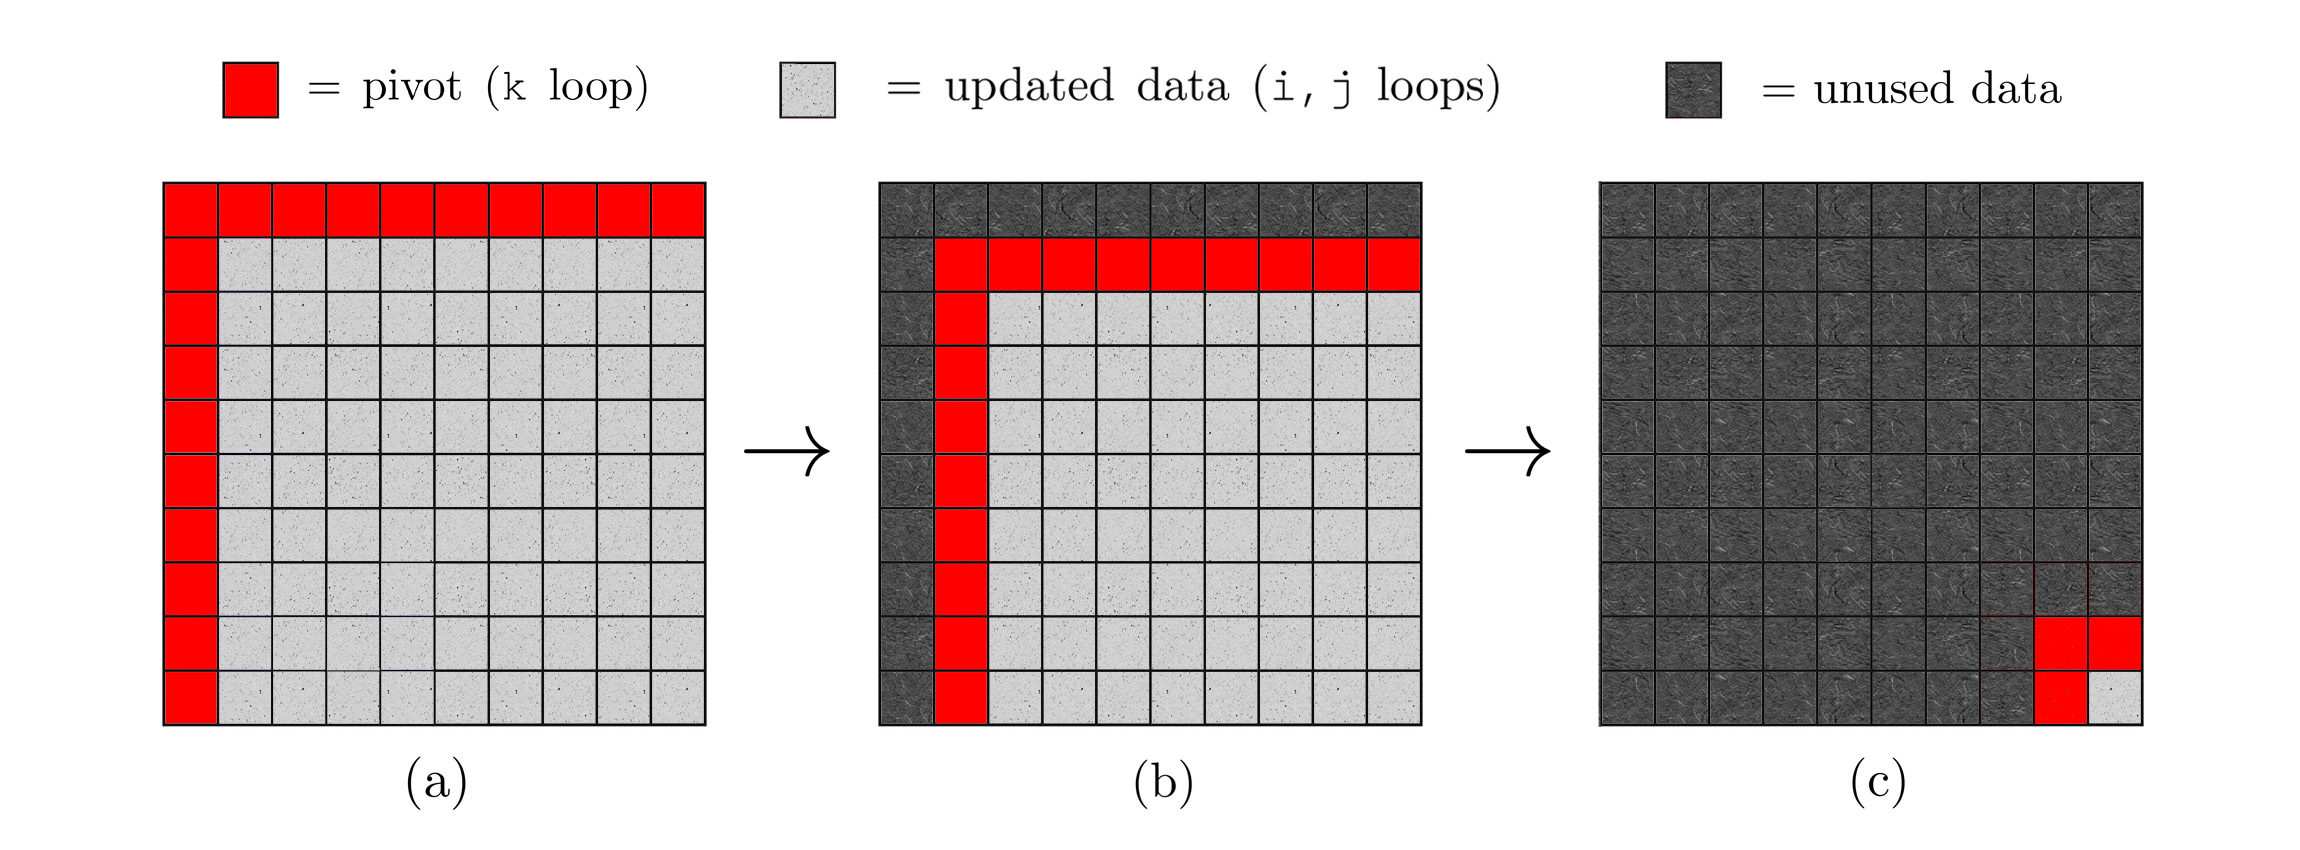
\includegraphics[scale=0.2]{algorithm.jpg}
\caption{Graphical representation of forward elimination algorithm based on~\cite{graph} for (a) the first iteration, (b) the second iteration, and (c) the final iteration.}
\label{algorithm}
\end{figure*}

\section{results}
\label{results}
For all three algorithms that have been developed, we analyze the performance by the CPU time as well as the number of FLOPs required as a function of matrix size. In addition, we analyze the accuracy of the algorithms by investigating the error as described in the previous section. Finally, we compare the performance of our developed algorithms to that of the LU decomposition.


\begin{table}[h]
\centering
\begin{tabular}{|c|c|}
\hline
$log_{10}(h)$ & $max(\epsilon_i)$\\
\hline
-1&-1.1797\\
-2&-3.08804\\
-3&-5.08005\\
-4&-7.07929\\
-5&-9.00487\\
-6&-6.77135\\
-7&-5.96231\\
\hline
\end{tabular}
\caption{Relative error as a function of step size}
\label{err_table}
\end{table}

\begin{table}[h]
\centering
\begin{tabular}{|c|c|}
\hline
algorithm& FLOPs\\
\hline
gauss&\\
tridiag&\\
specific&\\
LU  decomp&\\
\hline
\end{tabular}
\caption{Comparison of number of FLOPs for each algorithm.}
\label{flop_table}
\end{table}

\begin{figure}[t]
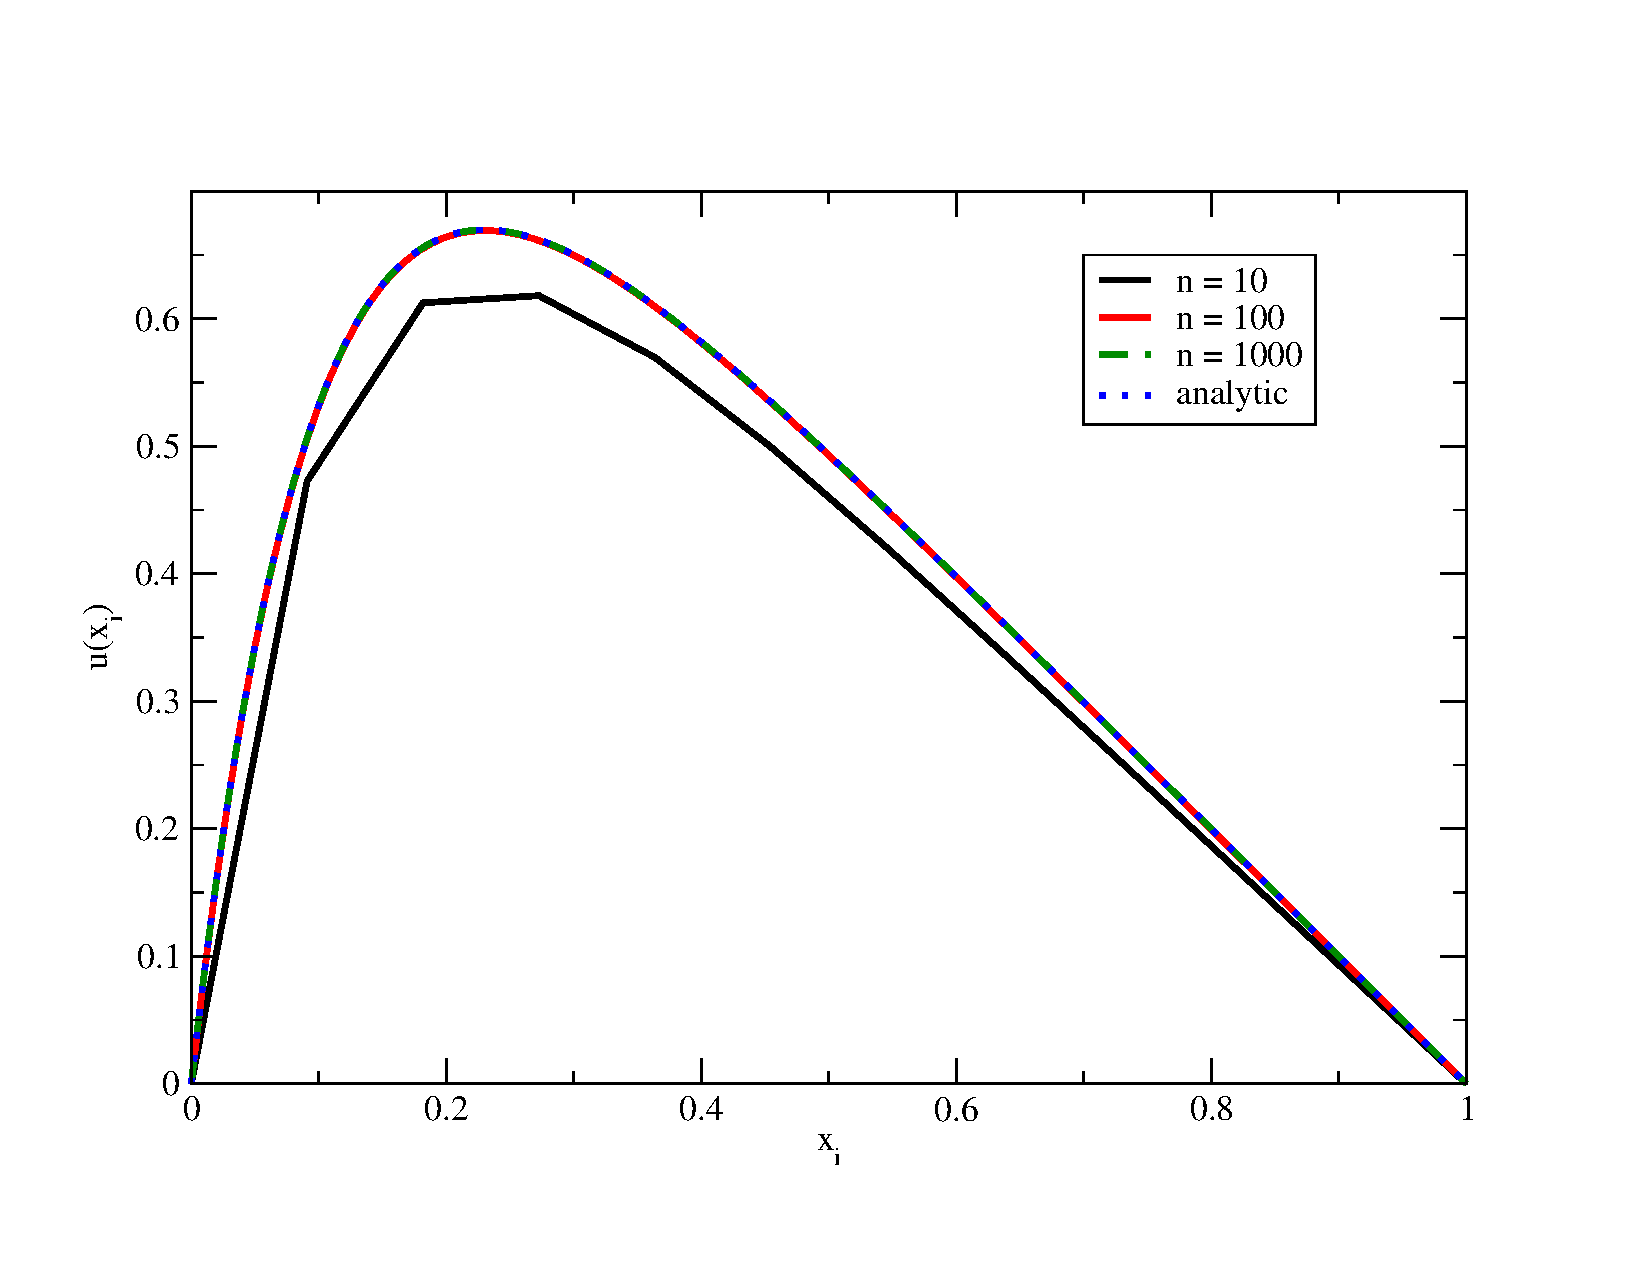
\includegraphics[scale=0.35]{output}
\caption{Solution to diff eqn as a function of matrix size}
\label{output}
\end{figure}

\section{conclusions}
\label{conc}

\bibliography{gauss}
\end{document}

